\documentclass{article}
\usepackage{v-test-paper}
\newenvironment{solution}{\par\noindent\color{red!85!black}$\Rightarrow$\vspace{0em}}{}
\renewcommand{\ans}{\quad}
\def\ansint#1{\quad}
\title{\textsc{NAIET-2024 Physics Paper Set B}}
\date{}
\ctikzset{batteries/scale=0.6}
\ctikzset{resistors/scale=0.6}
\begin{document}
\maketitle
\begin{enumerate}
    \item There are four vectors $\vec{a}$, $\vec{b}$, $\vec{c}$ and $\vec{d}$ are such that these represent the sides of a square with non-zero area as shown in the figure. Find the value of $\vec{a}+\vec{b}+\vec{c}+\vec{d}$.
        \begin{center}
            \begin{tikzpicture}
                \draw[->] (0,0) -- (2,0) node[mb]{$\vec{a}$};
                \draw[->] (2,0) -- (2,2) node[mr]{$\vec{b}$};
                \draw[->] (2,2) -- (0,2) node[ma]{$\vec{c}$};
                \draw[->] (0,2) -- (0,0) node[ml]{$\vec{d}$};
            \end{tikzpicture}
        \end{center}
        \begin{tasks}(4)
            \task $4\vec{a}$
            \task $2\left(\vec{a}+\vec{b}\right)$
            \task $4\vec{b}$
            \task None of these \ans
        \end{tasks}

    \item \[ s = ab + \dfrac{1}{2}at^2 \]
        In the above equation, if $s$ represents the displacement and $t$ represents the time, then what does $b$ represent?
        \begin{tasks}(4)
            \task Velocity
            \task (Displacement)$^2$
            \task (Time)$^2$ \ans
            \task None of these
        \end{tasks} 

    \item A body is moving in a circular path with a constant speed. Which of the following is statement is true about the particle ?
    \begin{center}
        
\begin{tikzpicture}
            \draw (0,0) circle (1);
            \fill (0,0) circle (1pt);
            \tzcoor*(45:1)(P)
            \tzline+[->](P)(135:1)
        \end{tikzpicture}
    \end{center}
        \begin{tasks}(1)
            \task It is moving with a constant velocity
            \task It is moving with a constant acceleration
            \task Its displacement remains constant between any equal intervals of time 
            \task None of these \ans
        \end{tasks}

    \item A block of mass $1 \kg$ is hanged from the ceiling using a massless string as well as tied to a completely horizontal massless string as shown in the figure. The block is in equilibrium. Find the tension in the horizontal string. (Take $g = 10 \mpss$)
        \begin{center}
            \begin{tikzpicture}
                \pic[rotate=180] (O) at (0,0) {frame};
                \node[block, anchor=north] (block) at (0, -2) {$1 \kg$};
                \pic[rotate=90] (P) at ($(block.east)+(2, 0)$) {frame};
                \tzline(block.east)(P-center)
                \tzline(block.north)(O-center)
            \end{tikzpicture}
        \end{center}
        \begin{tasks}(4)
            \task $10 \N$
            \task $5 \N$
            \task $2.5 \N$
            \task None of these \ans
        \end{tasks}

    \item A chain of mass $m$ and length $l$ is placed on a smooth horizontal surface. Now, this is chain in lifted slowly from one end to the vertical position. Find the work done by the person to lift the chain to the vertical position.
    \begin{center}
        \begin{tikzpicture}
            \pic (O) at (0,0) {frame=8cm};
            \foreach \x in {-1, -0.6, ..., 1} {
                \tzellipse[thick]($(O-center)+(-2 + \x, 0.1)$)(0.25 and 0.1)
                \tzellipse[thick]($(O-center)+(2, 1.25+\x)$)(0.1 and 0.25)
            }
        \end{tikzpicture}
    \end{center}
        \begin{tasks}(4)
            \task $mgl$
            \task $\dfrac{mgl}{4}$
            \task $\dfrac{mgl}{2}$\ans
            \task None of these 
        \end{tasks}

    \item Three positive equal charges $q_0$ each are placed at the vertices of an equilateral triangle as shown in the figure. Another charge $q$ is placed at the centroid of this triangle so that this system is in equilibrium. Find the value of $q$ in terms of $q_0$.
        \begin{center}
            \begin{tikzpicture}
                \foreach \A/\a/\p in {0/0/180, 0/3/0, 60/3/90} {
                    \tzcoor*(\A:\a)(P){$q_0$}[\p]
                    \tzline[dashed](P)(0,0)
                }
                \tzline[dashed](0:3)(60:3)
                \tzcoor*(30:{1.5*2/sqrt(3)})(C){$q$}
            \end{tikzpicture}
        \end{center}
        \begin{tasks}(4)
            \task $+q_0$
            \task $-q_0$\ans
            \task $+3q_0$
            \task None of these
        \end{tasks}


    \item In the given circuit, find the current $I_1$ flowing through the circuit.
        \begin{center}
            \begin{tikzpicture}
                \draw (0,0) to[battery, l_=$6 \V$] ++(4,0) to ++(0, 1.5);
                \draw (0,0) to ++(0, 1.5) to[R, l_=$6 \Ohm$, i_=$I_2$, invert] ++(4,0);
                \draw (0,0) to ++(0, 2.5) to[R, l_=$3 \Ohm$, i_=$I_1$, invert] ++(4,0) to ++(0, -1);
            \end{tikzpicture}
        \end{center}
        \begin{tasks}(4)
            \task $1 \A$ 
            \task $2 \A$ \ans
            \task $3 \A$
            \task None of these
        \end{tasks}

    \item Heat taken by a gas in process \( a-b \) is \( 6p_0V_0 \). Match the following columns.
        \begin{center}
            \begin{tikzpicture}
                \tzaxes(0,0)(4,3){$V$}{$p$}
                \tzline[-->--](1, 1)(2, 2){$b$}[ar]
                \tznode(1, 1){$a$}[bl]
                \tzline+[dashed](1, 1)(0, -1){$V_0$}[b]
                \tzline+[dashed](1, 1)(-1, 0){$p_0$}[l]
                \tzline+[dashed](2, 2)(0, -2){$2V_0$}[b]
                \tzline+[dashed](2, 2)(-2, 0){$2p_0$}[l]
                \tzline[dashed](0, 0)(1, 1)
            \end{tikzpicture}    
        \end{center}
        \begin{center}
            \renewcommand{\arraystretch}{1.5}
            \begin{table}[h]
                \centering
                \begin{tabular}{p{0.25cm}p{7cm}|p{0.25cm}p{4.5cm}}
                \hline
                & Column I & & Column II \\
                \hline
                (a) & \( W_{ab} \) & (p) & \( 4.5 p_0V_0 \) \\
                (b) & \( \Delta U_{ab} \) & (q) & \( 1.5 p_0V_0 \) \\
                (c) & Molar heat capacity in given process & (r) & \( 2R \) \\
                (d) & \( C_V \) of gas & (s) & None of these \\
                \hline
                \end{tabular}
            \end{table}
        \end{center}
        \begin{tasks}(2)
            \task $(a) \rightarrow (q), (b) \rightarrow (p), (c)\rightarrow (r), (d)\rightarrow (s)$ \ans
            \task $(a) \rightarrow (p), (b) \rightarrow (q), (c)\rightarrow (r), (d)\rightarrow (s)$
            \task $(a) \rightarrow (p), (b) \rightarrow (q), (c)\rightarrow (s), (d)\rightarrow (r)$
            \task None of these
        \end{tasks}


    \item A convex lens of focal length 20 cm produces images of the same magnification 2 when an object is kept at two distances \(x_1\) and \(x_2\) (\(x_1 > x_2\)) from the lens. The ratio of \(x_1\) and \(x_2\) is:
        \begin{tasks}(2)
            \task \(5 : 3\)
            \task \(2 : 1\)
            \task \(4 : 3\)
            \task \(3 : 1\)\ans
        \end{tasks}


    \item The logic gate equivalent to the given logic circuit is:
    \begin{center}
        \begin{tikzpicture}[circuitikz/logic ports=ieee]
            \draw (0,0) node[nand port] (A) {};
            \draw (-3, 1) node[not port](B) {};
            \draw (-3, -1) node[not port] (C) {};
            \draw (B.out) -- ++(1, 0) |- (A.in 1);
            \draw (C.out) -- ++(1, 0) |- (A.in 2);

            \tzcoor*($(B.in)+(-1, 0)$)(B')
            \tzcoor*($(C.in)+(-1, 0)$)(C')
            \tzcoor*($(A.out)+(1, 0)$)(A')
            \tzline(A.out)(A'){$Y$}[r]
            \tzline(B.in)(B'){$A$}[l]
            \tzline(C.in)(C'){$B$}[l]
        \end{tikzpicture}
    \end{center}
        \begin{tasks}(2)
            	\task NOR
            	\task NAND
            	\task OR \ans
            	\task AND
        \end{tasks}

\end{enumerate}
\end{document}
